% =====================================================================
% Regeneron STS 2027 Research Report
% Format: single column, 12 pt, Times, 1.5 line spacing, 1 in margins.
%
% NOTE ON SPACING: \onehalfspacing sets Word-style 1.5 (baselinestretch
% ~1.24 at 12 pt), which is what most graders mean by "1.5 spacing."
% If STS means a literal 1.5x baseline, swap it for \setstretch{1.5}.
% Verify by measuring a rendered page: 25-26 lines/page = Word 1.5,
% 22-23 lines/page = literal 1.5.
%
% NOTE ON SECTION NUMBERING: sections are forced to Roman numerals so
% that every cross-reference resolves to the same string it did in the
% IEEEtran version (e.g. "Section V" for Discussion). Do not change
% \thesection without re-reading the prose for hard-coded numerals.
%
% NOTE ON FLOATS: the IEEEtran version combined Table I, Table II and
% Fig. 2 into a single float to keep them together in one column. That
% construct is unnecessary in a single-column layout, so they are three
% separate floats here. Declaration order is preserved, so Fig. 1-4 and
% Table I-II carry the same numbers as before.
% =====================================================================
\documentclass[12pt]{article}

\usepackage[letterpaper,margin=1in]{geometry}
\usepackage{setspace}
\usepackage{amsmath,amssymb,amsfonts}
\usepackage{newtxtext,newtxmath}     % Times text and math -- must follow amssymb
\usepackage{graphicx}
\usepackage{booktabs}
\usepackage{caption}
\usepackage{textcomp}
\usepackage{xcolor}
\usepackage{url}
\usepackage{fancyhdr}
\pagestyle{fancy}
\fancyhf{} % Clear all header and footer fields
\fancyfoot[R]{\thepage} % Place the page number on the Right footer
\renewcommand{\headrulewidth}{0pt} % Remove the top header line
\renewcommand{\footrulewidth}{0pt} % Remove the bottom footer line


\captionsetup{font=small,labelfont=bf,justification=justified}
\renewcommand{\topfraction}{0.9}
\renewcommand{\bottomfraction}{0.8}
\renewcommand{\textfraction}{0.07}
\renewcommand{\floatpagefraction}{0.8}
\setlength{\parskip}{0pt}
\setlength{\parindent}{0.3in}

\renewcommand{\thesection}{\Roman{section}}

\title{\textbf{Conformal-Gated Surrogate Screening for N-1 Under-Voltage Contingencies: When Does a Conformal Gate Outperform Historical Baselines?}}

\author{Rajan Saha\\
\small Conestoga High School, Berwyn, PA, USA\\
\small Boston University RISE Data Science Practicum}



\date{}

\begin{document}
\maketitle
\thispagestyle{empty}\newpage

\setstretch{1.5}

% =====================================================================
\section*{Abstract}
\addcontentsline{toc}{section}{Abstract} 
Measuring the voltage after a single-element outage, or an N-1 screening, requires running an AC power-flow solve for each contingency. Running this power-flow solve is time-consuming. I propose a gate mechanism that ties a one-sided split-conformal lower-bound interval to the predicted minimum post-contingency voltage, certifying the contingency if the voltage is safe, flagging if unsafe, and escalating to the power-flow solve if it is unsure. In a pre-registered experiment, where I test how the boundary mass is affected by the generator setpoint floor (cases just above 0.94 get escalated, and the larger the share of cases in [0.94, 0.945) the higher the escalation rate, slowing speedup), I adjusted the baseline generator settings of the case118 grid, and the share of contingencies where the voltage is in [0.94, 0.945) dropped as predicted when I set the generator setpoint's lower bound at 0.96, with boundary mass (share of post-contingency voltages within [0.94, 0.945)) staying around the same at the setpoint floor of 0.93. On the case118 network, the gate from the gradient-boosted model misses $1.14 \pm 0.96$\% of violations at its held-out target (worst split 3.03\%; 4 of 5 splits $\leq$ 1\%), and is 1.44 times faster (speedup B) than the traditional solver. At the same solve budget, the gate performed roughly the same as the conditional-history (COND-HIST) baseline on case118 and Illinois-200 (pre-registered primary test — only tied after implementing a post hoc rule), and beats COND-HIST on case30 (99.26\% vs.\ 89.81\%) and case24 (98.85\% vs.\ 97.18\%), and the case24 result depends on the post hoc tolerance rule. On case118, the model's ranking catches more violations than a fixed static ranking only at small solve budgets. In N-2 contingencies, or two-element outages, after calibrating the band on N-1 contingencies and testing on N-2 contingencies without recalibration, the coverage falls from 0.9050 to 0.8394, with a pre-set formula resulting in a threshold of 0.8861. Some limitations include the use of only 4 networks and a synthetic sampler.


\vspace{0.15in}
\noindent\textbf{Keywords:} contingency screening, conformal prediction,
power-flow surrogate, selective prediction, power system security

% =====================================================================

\thispagestyle{empty}\newpage

\setcounter{page}{1}


\section{Introduction}
\label{sec:intro}

Power grids must be able to stay operational even if they lose the functionality of a single element. The N-1 criterion, for all the elements that might fail, determines whether the calculated voltages of the remaining components stay within safe operating ranges after an element fails \cite{nerc}. Normally, the check itself comes from a physics calculation called an AC power flow solve, run for each potential contingency. For a complex network with hundreds of elements, the solver becomes time-consuming and computationally expensive.

One method to improve performance is to replace the slow physics solver with a fast approximation. However, the fundamental issue with this approach is that it fails undetected, declaring an unsafe contingency safe, since it only provides a single-point estimate without any confidence or uncertainty interval \cite{bates2021}. As a result, the operator skips the slow solver and misses the unsafe scenario altogether. In addition, since the error is asymmetric, predicting too high certifies an unsafe condition as safe, which is a dangerous operational risk, while predicting too low inefficiently increases solver time. I add the solver time for escalated cases to the screening gate's total time to reflect the true end-to-end cost.

There have been several approaches when it comes to employing surrogate models for N-1 contingency tests. Manoharan \cite{manoharan2026} utilized a linear LODF screen, a standard physics approximation, that checks if any single piece of equipment in the N-1 test has any thermal overloading. To confirm its reliability, the system also runs randomized full solves on some of the equipment to ensure the method's validity. Alc\'antara and Chatzivasileiadis \cite{alcantara2026} use an AI foundation model and conformal prediction to create a binary yes/no switch for each line to determine whether there's a present risk or not for line loading. Christianson et al. \cite{christianson2025} designed an input-convex network that completely removes false negatives, although that claim is only relevant to DC power flow models, not the AC power flow model my study uses. My work stands out from these papers in three distinct ways. First, unlike Manoharan's approach, I add a per-case one-sided safety margin to each numerical voltage prediction made by the models. Second, I tested the boundary mass (the share of voltages in [0.94, 0.945)) on the original builds and successfully replicated on the rebuilt data how it responds to the lowest allowed generator setting. Third, I compare my models against a conditional-history (COND-HIST) baseline (a no-machine-learning-history algorithm that is conditioned on the pre-outage margin), given the same solve budget. I investigate three questions: does a conformal gate beat a COND-HIST baseline using the same solve budget (limited number of power flow solves); does the same target coverage (measure of band's reliability) calibrated on N-1 contingencies maintain its reliability under N-2 contingencies, or two-branch outages; and does moving the generator setpoint floor change the boundary mass in the way predicted in advance?

% =====================================================================
\section{Background}
\label{sec:background}

A per-unit (pu) voltage normalizes power grid values into simple decimals (where 1.0 is nominal), where 0.94 pu indicates a 6\% under-voltage. Utilities must keep voltage within a band around nominal, and this study flags any part of the grid that fails the test against an under-voltage limit of 0.94 pu. The N-0 condition represents the current state of the grid without any equipment outages. In my experiment, I kept all voltages above the 0.94 pu limit. I refer to this pre-outage state of the grid as a base case. However, if a single piece of equipment fails, the rest of the network must absorb the extra load, which could cause the voltage at one or more buses to go under the safe 0.94 pu limit. N-1 screening simulates these failures and detects any violations of the under-voltage limit before they happen. In this study, I do not check for overvoltage, although in 73.38\% of converged N-1 rows, the highest bus voltage is over 1.05 pu. Also, the gate only bounds one predicted scalar, so adding more factors would require their own respective target and bands. I cannot check for thermal loading because case118 assigns every line the same 9,900 MVA rating, which is a placeholder value that is not realistic, so the test would pass every case regardless of conditions \cite{pypower}.

An AC power flow solver is used to get the final voltages across a network after a single-element failure. Due to the math being complex and non-linear, it takes around 9 milliseconds for one scenario on an Apple M5 processor, and the time multiplies across all the contingencies. By contrast, a prediction from a machine learning model can take a fraction of a millisecond to predict the single minimum voltage out of the whole grid. Classical fast screens rank contingencies using the current operating conditions without running a full solver \cite{ejebe1979}, which contrasts with what the static ranking baseline does in my experiment, as the static ranking baseline ranks which contingency is the most dangerous to the grid and is a fixed offline list. While the static ranking baseline ranks which contingency is the most dangerous in a grid, it fails to provide a numerical minimum voltage.

I study the IEEE 118-bus system \cite{case118}, a standard electrical power test case with 118 buses (the junctions where voltage is measured), 173 lines, and 13 transformers. Since the contingencies set includes only lines and transformers, there are 186 total pieces of equipment that are subject to failure. Each contingency subjects a single line or transformer to failure. Some base cases are also missing a generator before the contingency, so those rows have two elements out after it, which I describe in Section~\ref{sec:method}. I also study the Illinois-200 \cite{illinois200}, case30 (regenerated version, as the original version had line overloading, as stated in Section~\ref{sec:method}) \cite{case30}, and IEEE RTS case24 bus systems \cite{case24}, each having 200, 30 and 24, buses respectively, and 245, 41, and 38 branches, respectively. I use pandapower \cite{pandapower}, a Python library used to model power systems, for solving post-outage voltages while ensuring specific generator reactive power limits are enforced. Handling these limits required some adjustments made to the method pandapower manages them, as stated in Section~\ref{sec:method}.

% =====================================================================
\section{Method}
\label{sec:method}

\subsection{Dataset}\label{subsec:dataset}

I determined the load levels by scaling the initial network load of the case118 network by multipliers. For Independent mode (750 bases), I multiplied the load by multipliers ranging from 1.0 to 1.12. For Regional mode (750 bases), I did the same but from 0.9005 to 1.2317 (43.65\% outside the 1.0 to 1.12 target range), while reactive power scales across all 1,500 bases range from 0.8146 to 1.4065 (to account for stochastic variations in the random power factor). The base cases were kept if the minimum pre-outage voltage was above 0.94 pu. Before this check, I removed one generator (never the slack generator) 30\% of the time. Since weaker grids failed the check more often, 431 of the 1{,}500 kept bases (28.73\%) have a generator that is out of service. Each accepted base case was put through a simulation of 186 contingencies representing single-element failures, followed by an alternating-current power flow calculation to determine the minimum bus voltage after each contingency. The total sample contained 1{,}500 base cases and 280{,}500 rows, including the base cases. Out of those rows, 1{,}500 were N-0 base rows that were excluded because they are not contingencies, while the other 279{,}000 rows are N-1 contingencies. Out of those 279{,}000, 55 were removed due to failing to converge, resulting in 278{,}945 converged rows. Minimum post-contingency bus voltages ranged from 0.7605 to 0.9594 per unit, and 16.26\% of the observations violated the voltage limit. 

The previous implementation of the dataset generator used a lower bound of 0.94 pu for voltage set points and truncated any set points that fell below that lower bound value at the threshold (in an earlier build before the switch-back fix, described in the next paragraph). That resulted in a cluster of samples near $0.940000 \pm 1\times10^{-9}$ per unit, which accounted for 35.17\% of the converged rows, due mainly to bus 76, which was a generator bus and had a base voltage set point of 0.943 per unit. I discovered the problem after inverting the escalation versus band width relation, which returned unattainable accuracy requirements. After modifying the code and resampling the data, the exact spike at 0.940000 per unit went away, but the number of rows in the narrow band [0.94, 0.945) stayed about the same, moving from 55.5\% to 56.86\% (55.5\% is from the earlier clipped build and 56.86\% is from the original build, and the rebuilt build with the switch-back fix is 54.75\%). The current grid still uses the same generator setpoint floor of 0.94 pu, and now they are within $\pm$0.025~pu of the generator's base setpoint, with any draw outside 0.94--1.06~pu redrawn instead of setting it to 0.94 pu as before.

As for the switch-back fix, pandapower handles generator reactive power (Q) limits in one direction, meaning that once the generator reaches its Q limit, it fails to maintain a proper voltage and is not switched back to voltage control when a generator held at either Qmax (back to voltage control when bus voltage > setpoint) or Qmin (when bus voltage < setpoint). To fix this, I added a loop (switch-back rule) that switches the generator back to voltage control based on its setpoint, and rebuilt every dataset with this change. To check this on the original build, I used MATPOWER, another open-source electric power system simulation widely used by power system researchers \cite{matpower}, testing 201 labels, or the minimum voltages among the buses connected to the slack bus. Of the 201 labels from the new switch-back fix, 100 were sampled from a total of 4,615 labels that changed from violation to safe, and another 100 were sampled from a total of 2,162 labels that changed from safe to violation, and 1 was chosen as the worst case (the bus at 0.8485 pu in my earlier results). MATPOWER, without this rule, returned the same old label (0.8485 pu).  MATPOWER's labels, once run with the switch-back rule as before, matched all 201 of 201 corrected switch-back labels, with the worst case's voltage at 0.94507 pu (originally 0.8485 pu under the old one-way Q-limit handling), which is now safe. After running a separate power-flow solver on the rebuilt datasets to recompute sample rows from each dataset, all 10 datasets passed the preset check, with all but 4 rows (2 in case24, 1 in the 0.93-floor build, and 1 in the N-2 data — excluding trafo 63) matching the rebuilt datasets’ own labels. In addition, the 200 rows near the limit matched in every dataset to the separate solver, with Illinois passing, and the 3 trafo-63 rows being counted as failures and not part of the 200 near-limit rows. In case118, there were 9 outages (4.84\% of rows), Illinois had 71 outages (29.69\% of rows, excluding trafo 63), case30 had 3 outages (7.32\% of rows), and case24 had 1 outage (2.73\% of rows). These outages split each grid into islands, and the solver evaluated the buses that are still connected to the slack bus; any buses not connected to the slack bus are left out by the label, so the gate does not check the load on those buses.

I also tested the published IEEE case30 system, where the published base case is at 111.83\% line loading, which is discussed in Section~\ref{sec:discussion}. Because that loading is unrealistically high, I regenerated the case30 network by keeping only the base cases that have the maximum line loading of at most 100\% and lowering the load-multiplier window to 0.87--0.99, which brought the maximum base-case line loading down to just under 100\%. Since there are 41 rather than 186 branches, the 1{,}500 bases produce 61{,}500 contingency scenarios, all of which were solved and converged successfully. I also tested the Illinois-200 synthetic network, which has 200 buses and 358,694 converged rows after trafo (transformer) 63 is removed. I removed trafo 63 as having a contingency on this equipment isolates 199 buses and all 37 generators into an island, or buses that are completely disconnected from the slack bus. Since the label for trafo 63 is always 1.04 pu as it is just the voltage from the slack bus, it is classified as safe while the cut off buses are not accounted for. I then created a post hoc rule stating that if an island is created from a contingency, the island cut off from the slack bus must have fewer than half of the buses to be a valid contingency that I count in my results. Only trafo 63 fails these requirements as every other islanding outage on all four networks keeps at least 95.8\% of buses connected to the slack bus. Finally, I also tested the case24 network, with 24 buses and 53,498 rows. On case24, 6.14\% of the rows (3,502 of 57,000) and 1.99\% of the rows (7,306 of 367,500) on Illinois-200 were dropped due to them not converging, as specific equipment like case24's line 8 and line 25 from Illinois-200 fail in every base case. When I re-built the data from each network with the new switch-back mechanism from the solver, I set a pre-registered check to ensure the values matched before and after the re-run, and stopped and reported the network if it has over 0.5\% of rows that fail the switch-back solve. Due to computer rounding, case24 failed the exact-match check by at most $1.95\times10^{-14}$~pu, while the switch-back labels matched exactly. After seeing this, I added another post hoc rule stating that a value within $10^{-9}$~pu was allowed. In addition, there was no rebuilt gate versus baseline result at the time for case24 when this post hoc was added, and on the original-data case24 build the gate beat COND-HIST. Before I added this tolerance rule, I had an earlier analysis which already computed case24 safety numbers (missed rate, escalation, speedup) on the original case24 base cases with its corrected inputs. Also, I excluded the testing of the case39 network as 1.09\% of its rows failed the switch-back solve, which is above the 0.5\% threshold I set initially.

\subsection{Surrogates}

The surrogate predicts the minimum voltage following an outage based on the per-bus loads, how generators are set up, baseline voltages, and the failed equipment. The two algorithms used in this study are a ridge linear regression model using standardized inputs and a histogram-based gradient-boosted tree ensemble \cite{sklearn}. The dataset is split into 60\%, 20\%, and 20\% sets using different base scenarios for training, calibration, and test sets, respectively. To tune the specific variables for each model, I split the training set again into three smaller parts: one to fit the model, one to calculate the band width $\hat{q}$, and one to test the gate on, ensuring there is no data leakage between these three and the real calibration or test sets when choosing variable values. I selected the hyperparameters and coverage target that skipped the most solves while still missing 1\% or fewer of the violations, and I repeated the whole process with five different random splits. I tested these models by first getting the held-out operating points from the inner tuning split data and then testing the held-out operating points once on the test set. As a result across all the splits, the mean coverage target for ridge was 0.934$\pm$0.010 and 0.970$\pm$0.011 for histgb (the gradient-boosted model). I tested my models against two simple and three history baselines: persistence, which predicts the pre-outage minimum voltage; training mean, which takes the mean voltage in the training data; fixed static ranking, which ranks contingencies by the amount of violations they caused in the training data and has the same number of solves per base case; conditional-history (COND-HIST) baseline, a no-machine-learning-history algorithm to rank outages by observing the pre-outage voltage margin and the outaged line; and global-budget static ranking (GLOBAL-STATIC), which uses the same fixed list as fixed static ranking, but some base cases are allowed to run more solves than others. Persistence and training mean replace the models using the same gate the model uses, as defined in Section~\ref{subsec:gate}. I also define the catch rate of the models as $1-{}$missed rate, where the flagged cases are solved. In addition, the three history baselines defined above get a solve budget (limited number of power flow solves) that equals the total number of solves the gate used.

\subsection{One-sided conformal band}

The split-conformal prediction approach converts the residuals from the calibration dataset into a coverage guarantee (the probability that the true voltage is at or above the band's lower end)\cite{lei2018,vovk2005,angelopoulos2023}. Since the primary source of the danger is the voltage being less than the predicted one, I compute only the lower band. It is specified via $\hat{q}$ as the quantile for the coverage of the model overshoot (the difference between the prediction and the true value) based on the finite-sample rank approach proposed by Lei et al.\ \cite{lei2018}, and forms the one-sided band
\begin{equation}
\text{lower} = \hat{p} - \hat{q},
\end{equation}

where $\hat{p}$ is the prediction. As long as the test cases and calibration cases are exchangeable (in this case drawn the same way with the same distribution — this guarantee is only an approximate coverage, as $\hat{q}$ is the quantile over all calibration rows, and 186 rows from a base case are correlated), the true voltage remains at or above the lower bound with the desired probability that is accurate on average across various test rows. If this condition does not hold (e.g., using calibration data of a single-element outage and test data where two branches fail together), there is no guarantee for what the band truly encompasses, which raises the issue of distribution shift described in Section~\ref{sec:discussion}. A single quantile coverage is the easiest way to choose the band, and there are locally adaptive alternatives that exist \cite{romano2019}. The held-out calibrated band widths are 0.0062$\pm$0.0008 per unit for the linear model and 0.0051$\pm$0.0010 per unit for the gradient-boosted model, with mean targets of 0.934 for ridge and 0.970 for histgb.

\subsection{Three-way gate}\label{subsec:gate}

For each contingency, the gate performs the following tests for the band and the point prediction compared with the limit $L=0.94$:
\begin{itemize}
\itemsep0em
\item \textbf{Certify} (skip the solver): $\hat{p}-\hat{q}\ge L$, meaning that the lower edge of the band exceeds the limit.
\item \textbf{Flag} (skip the solver): $\hat{p}< L$, meaning that the point prediction itself is below the limit.
\item \textbf{Escalate} (invoke the solver) otherwise, that is, when the band straddles the limit.
\end{itemize}
The flagging test employs the point prediction, since the lower edge of the one-sided band has no upper edge (Fig.~\ref{fig:gate}). In the equations below, both speedup A and B equations account for the time the invoked solver takes on escalated cases, while speedup B also accounts for solver time on flagged cases:
\begin{align}
\text{speedup}_A &= \frac{n\, t_{\text{solve}}}{n\, t_{\text{surr}} + n_{\text{esc}}\, t_{\text{solve}}}, \label{eq:speedupA}\\
\text{speedup}_B &= \frac{n\, t_{\text{solve}}}{n\, t_{\text{surr}} + \left(n_{\text{esc}} + n_{\text{flag}}\right) t_{\text{solve}}}. \label{eq:speedupB}
\end{align}
Here $n$ is the total number of contingencies, $n_{\text{flag}}$ is the total number of flagged contingencies, $t_{\text{solve}}$ is the solver time per case (set at 9.14 ms on the M5 processor on the case118 network, which is the minimum over 400 timed solves), $t_{\text{surr}}$ is the surrogate time that excludes the time for feature building ($0.00173\pm0.00074$~ms for ridge and $0.00919\pm0.00527$~ms for histgb per case, timed as one batch prediction divided by the number of cases), and $n_{\text{esc}}$ is the escalation count. Using base-case voltages requires an extra solver run per base case, which slows down the speedup slightly, and the solver time I used was 9.14 milliseconds, which is the fastest run out of 400 runs, making the speedup conservative. For the main results, the speedup B equation is used as in real world scenarios, an operator would double check the flagged scenarios before acting upon them. This makes Tables~\ref{tab:networks} and~\ref{tab:budget} in Section~\ref{subsec:gatevsbaslines} a comparison of how well each method ranks cases. The speedup for the speedup B equation is close to the inverse of the escalation rate plus the flag rate since the surrogate is much cheaper than the solve.

% ---------------------------------------------------------------------
% FIGURE 1 (fig:gate) -- gate schematic. Cited in III-D.
% ---------------------------------------------------------------------
\begin{figure}[htbp]
\centering
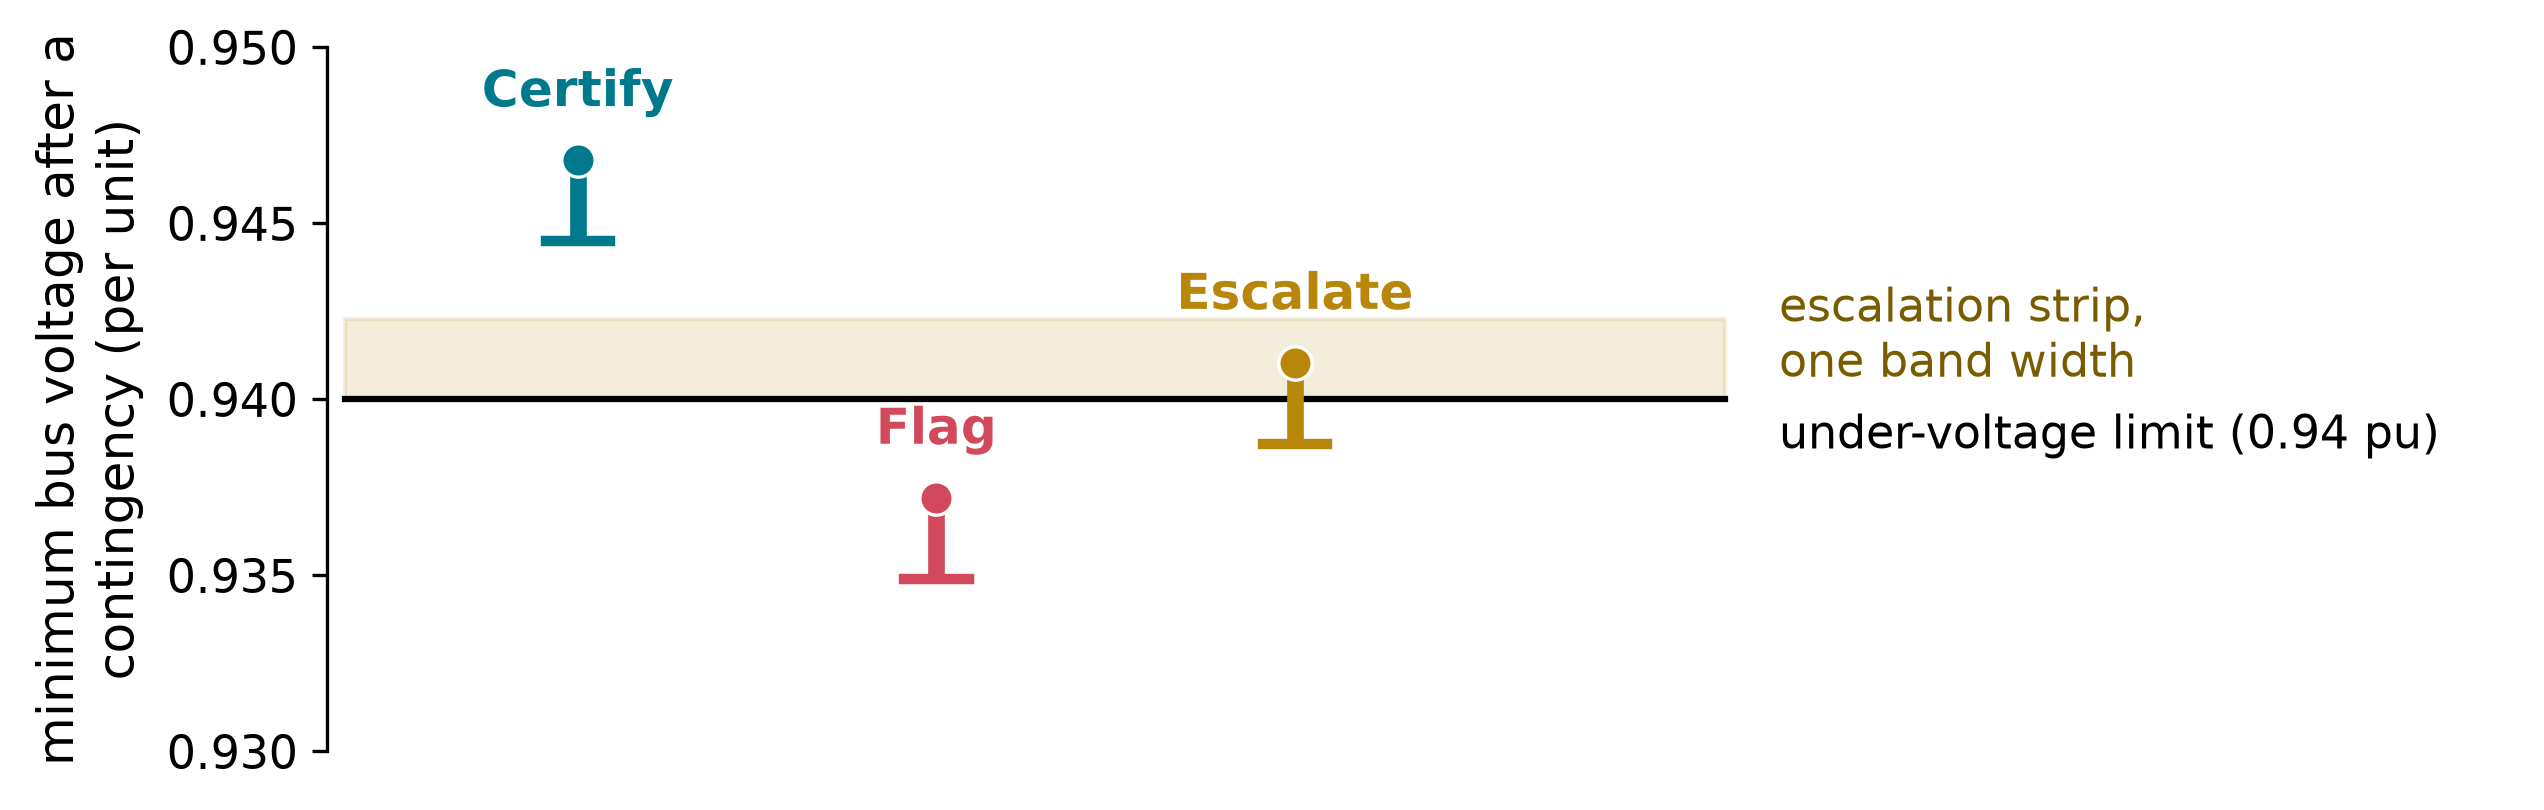
\includegraphics[width=0.65\textwidth]{data/gate_schematic_v4.png}
\caption{The three-way gate mechanism is shown above. The band extends only downward, since the main risk I am screening for is the true voltage sitting below the prediction. A case is certified, and the solver is skipped when the whole band clears 0.94 pu; flagged and the solver is skipped when the point prediction falls below it; and escalated to the exact solver when the band straddles the limit.}

\vspace*{1ex}
{\scriptsize Graph created by Rajan Saha using Matplotlib 3.11.1, 2026}


\label{fig:gate}
\end{figure}


\subsection{Theory}\label{subsec:theory}

Escalation happens when the model predicts in the same interval where the band crosses the threshold. This escalation behavior from the gate can be written as an equation. Let $L=0.94$ be the under-voltage limit, $\hat{p}$ be the surrogate prediction, and $\hat{q}$ be the calibrated one-sided conformal band width. A contingency is escalated when the prediction is inside the interval,
\begin{equation}
\mathbf{1}\{L \le \hat{p} < L + \hat{q}\},
\end{equation}
which lines up with the definitions of the gate's certify/escalate/flag mechanism.

Another relationship can be drawn from analyzing both the certification and true violation conditions from the gate's method. Certification from the gate requires $\hat{p} - \hat{q} \ge L$, which can be rewritten as $\hat{p} \ge L + \hat{q}$. In addition, a true violation results in $y < L$. Altogether, these give a calculation of the model's overshoot $o = \hat{p} - y$:
\begin{equation}
o \ge \hat{q} + (L - y),
\end{equation}
so the model's overshoot must be at least equal to the band width plus how far below the true voltage is from the limit, or $L - y$. The only way the model and the gate miss the violation is if the model overshoots by at least the band width plus the violation's depth.


\subsection{Experimental design and pre-registration}\label{subsec:prereg}

Before these experiments, I created the decision rule for the run and pushed it to GitHub for each later round of experiments before running them and collecting the results. Each pushed rule matches its own hash, proving it was not edited since it was hashed, and was pushed to GitHub before the results were returned from the experiment, further proving that it was made before the run. The two exceptions to this were running my first floor experiment, which had no GitHub record at the time due to not establishing this precedent and was committed after the run completed, and the 0.95-floor safety/speed tests, which were committed along with its respective results. The first results were decided from the original builds, and I rebuilt the data and re-ran the same tests to ensure consistency, making these new results replications on corrected data. The three questions listed below have a rule written down beforehand to determine their outcome:

\begin{enumerate}

\item \textbf{Does the gate beat COND-HIST at the same solve budget?} The rule for the gate to beat COND-HIST is that the gate's catch rate across splits must be higher than the catch rate of the baseline by more than the larger of these two rates' standard deviations across the five splits, and if the gap is smaller than the larger standard deviation, the result is a tie. This rule and Illinois-200 being chosen as the primary network were established before running the experiments.
\item\label{item:n2} \textbf{Does N-1 calibration of a 90\% promise stay reliable on N-2 outages?} The rule of the coverage holding only if the average N-2 coverage across the 5 splits is at least 0.90 minus the greater of the two split-to-split standard deviations, accounting for normal split-to-split variation, was set in advance. This design included 50 random branch pairs per base case of the N-2 contingencies with no retraining or recalibration on N-2 data. 
\item \textbf{Does moving the generator setpoint floor change the boundary mass as predicted?} I set the predictions of 55\% (range 50--62\%) at a floor of 0.93 and about 20\% (range 8--30\%) at 0.96 in advance. I tested this prediction on the original build and replicated this on the rebuilt data. For this to pass, the boundary mass must be more than 5 points below the 0.95 build on 0.96 and within 5 points of the 0.94 build at 0.93.
\end{enumerate}

What I did not decide in advance was the case24 tolerance of $10^{-9}$~pu and the trafo 63 exclusion from the contingency test, as well as the post hoc refit described in Section~\ref{sec:discussion}, dropping only case39, the Illinois validation and keeping stored inputs for 2 case24 bases in an earlier run.


% =====================================================================
\section{Results}
\label{sec:results}

Both surrogate models accurately predict the minimum post-contingency bus voltage used by the gate to make its decision. Tables~\ref{tab:models}, \ref{tab:ops}, \ref{tab:networks}, \ref{tab:budget} and \ref{tab:n2} are based on the rebuilt data that replicated the original build, with the original-build tests reported wherever they differ. The linear model reaches an $R^2$ of 0.815 and the gradient-boosted model 0.953, with mean absolute errors of 0.00344 and 0.00130 per unit, respectively (Table~\ref{tab:models}). At 90\% coverage, the ridge model escalates 47.28\% of cases, has 89.4\% coverage, misses 2.99\% of violations, and, using speedup A, is 2.13 times faster than the solver. The gradient-boosted model escalates 24.23\%, has 90.5\% coverage, and, using speedup A, is 4.18 times faster than the solver, yet it misses 4.06\% of violations. Both models aim to target the specific coverage for the band, as the coverage is close to 90\%. In addition to coverage, the only quantity targeted, I also measure missed rate, escalation rate, and speedup. The question of safety shifts from how many errors were made to where they occur.

% ---------------------------------------------------------------------
% TABLE I (tab:models) -- rebuilt (N13) values from
% data/sts_n13_compare.json -> rows[table=tab:models] -> rebuilt_mean/std.
% Speedup is speedup A (flagged cases not solved).
% ---------------------------------------------------------------------
\begin{table}[htbp]
\centering

\caption{Four-model comparison at 90\% target coverage. Means $\pm$ standard deviation over five random splits using Speedup A (flagged cases are not solved). Escalation and missed-violation rate (share of true violations) in percent; histgb is the gradient-boosted model. $^{\dagger}$Since the train-mean model calls the solver 100\% of the time, speedup is 1.00 as it takes the same amount of time the solver takes.}
\label{tab:models}
\small
\begin{tabular}{lccccc}
\toprule
Model & MAE ($10^{-3}$ pu) & $R^2$ & Esc. & Missed & Speedup A \\
\midrule
persistence & 3.90$\pm$0.05 & $-0.050\pm0.005$ & 98.40$\pm$0.74 & 1.16$\pm$0.57 & 1.02$\pm$0.01 \\
$^{\dagger}$train mean  & 6.29$\pm$0.14 & $-0.000\pm0.000$ & 100.00$\pm$0.00 & 0.00$\pm$0.00 & 1.00$\pm$0.00 \\
ridge       & 3.44$\pm$0.12 & 0.815$\pm$0.010 & 47.28$\pm$4.49 & 2.99$\pm$0.67 & 2.13$\pm$0.18 \\
histgb      & 1.30$\pm$0.17 & 0.953$\pm$0.007 & 24.23$\pm$3.35 & 4.06$\pm$0.73 & 4.18$\pm$0.53 \\
\bottomrule
\end{tabular}

\vspace*{1ex}
{\scriptsize Table created by Rajan Saha using Python and \LaTeX, 2026}
\end{table}


\subsection{Safety comes at high escalation}

In Table~\ref{tab:ops}, I adjusted the target from 0.90 to 0.98 and recorded the missed and escalation rates. Graphing the rate of misses versus the percentage of cases for which the gate solves the problem without the help of the solver provides the risk--coverage curve for selective prediction \cite{geifman2017,elyaniv2010} (where coverage is the acceptance rate). As the target gets larger, the missed rate decreases, but the escalation rate goes up because the band size has to be bigger to account for model overshoot. For the gradient-boosted model, increasing the target from 0.90 to 0.94 decreases the missed rate from 4.06\% to 2.36\%, increases the escalation from 24.23\% to 36.43\%, and decreases speedup A from 4.18 to 2.77 times. The ridge model shows a similar pattern as well, with the average of missed cases falling below 1\% at 0.95 for the ridge model (0.74\% missed, 67.18\% escalation, 1.49 times speedup A) and 0.98 for the gradient-boosted model (0.69\% missed, 63.39\% escalation, 1.58 times speedup A), although the error bars still reach up to about 0.97--1.07\%, as Fig.~\ref{fig:tradeoff} shows.

% ---------------------------------------------------------------------
% TABLE II (tab:ops) -- rebuilt (N13) values from
% data/sts_n13_compare.json -> rows[table=tab:ops] -> rebuilt_mean/std.
% Cov. = coverage_emp x 100. Held-out target is the mean +/- std of the
% per-split target chosen on the inner split.
% ---------------------------------------------------------------------
\begin{table}[htbp]
\centering
\caption{Safety and throughput at each coverage target on IEEE 118-bus system using speedup A (flags not solved) and speedup B (flags are also solved). Means $\pm$ standard deviation over five random splits. Escalation, empirical coverage, and missed-violation rate (share of true violations) in percent; histgb is the gradient-boosted model.}
\label{tab:ops}
\small
\setlength{\tabcolsep}{4pt}
\begin{tabular}{llccccc}
\toprule
Model & Target & Esc. & Cov. & Missed & Speedup A & Speedup B \\
\midrule
ridge  & 0.90 & 47.28$\pm$4.49 & 89.4$\pm$1.5 & 2.99$\pm$0.67 & 2.13$\pm$0.18 & 1.44$\pm$0.08 \\
ridge  & 0.94 & 62.54$\pm$2.80 & 93.8$\pm$0.6 & 1.16$\pm$0.28 & 1.60$\pm$0.07 & 1.18$\pm$0.05 \\
ridge  & 0.95 & 67.18$\pm$1.39 & 94.9$\pm$0.7 & 0.74$\pm$0.23 & 1.49$\pm$0.03 & 1.11$\pm$0.02 \\
ridge  & 0.96 & 71.63$\pm$2.42 & 96.0$\pm$0.3 & 0.42$\pm$0.20 & 1.40$\pm$0.05 & 1.06$\pm$0.02 \\
ridge  & 0.97 & 75.15$\pm$2.17 & 96.9$\pm$0.3 & 0.21$\pm$0.15 & 1.33$\pm$0.04 & 1.02$\pm$0.01 \\
ridge  & 0.98 & 76.89$\pm$2.10 & 97.9$\pm$0.1 & 0.11$\pm$0.13 & 1.30$\pm$0.04 & 1.01$\pm$0.00 \\
ridge  & held-out (0.934$\pm$0.010) & 59.47$\pm$5.91 & 93.4$\pm$1.3 & 1.51$\pm$0.60 & 1.70$\pm$0.17 & 1.23$\pm$0.10 \\
\addlinespace
histgb & 0.90 & 24.23$\pm$3.35 & 90.5$\pm$1.4 & 4.06$\pm$0.73 & 4.18$\pm$0.53 & 2.45$\pm$0.20 \\
histgb & 0.94 & 36.43$\pm$3.97 & 94.3$\pm$0.6 & 2.36$\pm$0.66 & 2.77$\pm$0.28 & 1.89$\pm$0.14 \\
histgb & 0.95 & 40.32$\pm$3.48 & 95.1$\pm$0.6 & 1.94$\pm$0.60 & 2.49$\pm$0.20 & 1.76$\pm$0.10 \\
histgb & 0.96 & 46.81$\pm$2.31 & 96.1$\pm$0.4 & 1.40$\pm$0.47 & 2.14$\pm$0.10 & 1.57$\pm$0.06 \\
histgb & 0.97 & 53.79$\pm$2.59 & 97.0$\pm$0.4 & 1.03$\pm$0.46 & 1.86$\pm$0.09 & 1.42$\pm$0.05 \\
histgb & 0.98 & 63.39$\pm$2.63 & 97.9$\pm$0.4 & 0.69$\pm$0.38 & 1.58$\pm$0.06 & 1.25$\pm$0.04 \\
histgb & held-out (0.970$\pm$0.011) & 54.25$\pm$9.68 & 97.0$\pm$1.4 & 1.14$\pm$0.96 & 1.91$\pm$0.41 & 1.44$\pm$0.23 \\
\bottomrule
\end{tabular}

\vspace*{1ex}
{\scriptsize Table created by Rajan Saha using Python and \LaTeX, 2026}
\end{table}




% ---------------------------------------------------------------------
% FIGURE 2 (fig:tradeoff) -- coverage sweep,
% data/sts_n13_fig2_tradeoff.png.
% ---------------------------------------------------------------------
\begin{figure}[htbp]
\centering
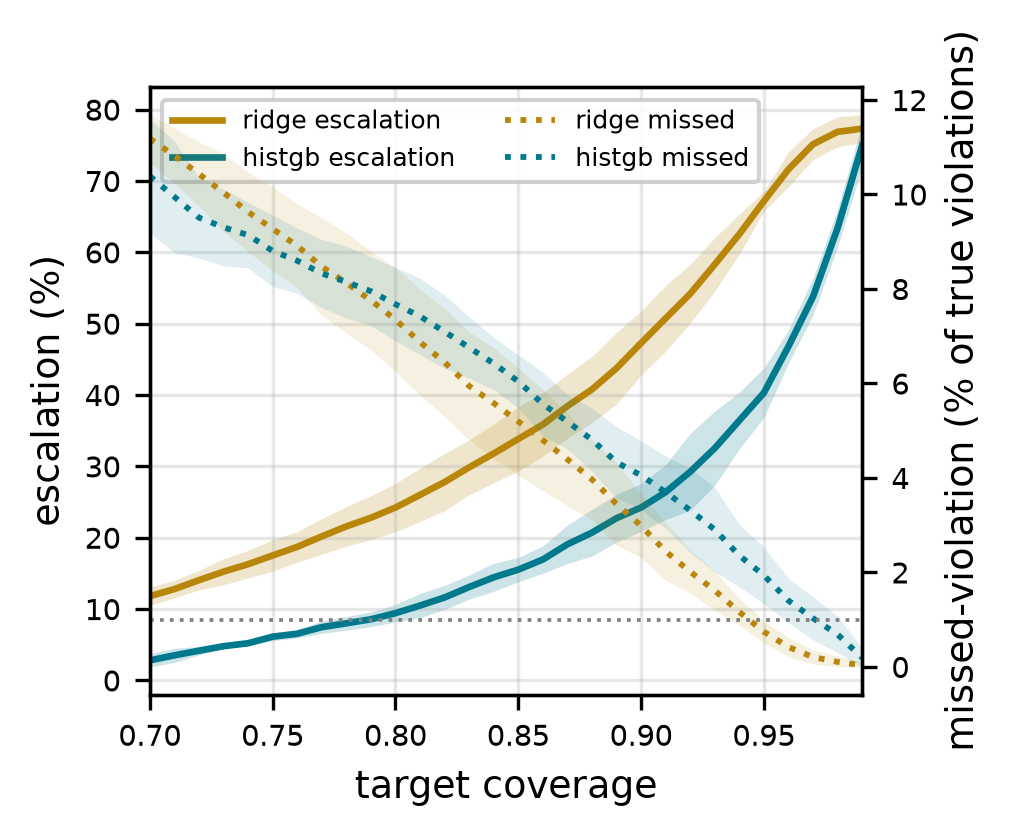
\includegraphics[width=0.5\textwidth]{data/sts_n13_fig2_tradeoff.png}
\caption{Escalation (solid, left axis) and missed violations (dotted, right axis) are plotted against the safety target and averaged over five splits. The mean missed rate first falls just under 1\% at 0.95 coverage for ridge and 0.98 for the gradient-boosted model, with high escalation at both and the error bars for histgb reaching slightly above 1\%.}

\vspace*{1ex}
{\scriptsize Graph created by Rajan Saha using Matplotlib 3.11.1, 2026}

\label{fig:tradeoff}
\end{figure}

Persistence is the baseline model where the voltage before the outage of one element is assumed to be equal to the voltage after it. All the pre-outage scenarios are above 0.94 pu, so its predictions never go below the limit, and since it cannot predict under the limit, it can never mark a case as a violation. In Table~\ref{tab:models}, the model escalates 98.40\% of cases and is barely faster than the solver in terms of time taken. An operator that requires a missed rate around 1\% (with error bars still touching the 1\% threshold) would run the models at a 0.95 or a 0.98 target coverage and accept about a 1.11 to 1.25 times speedup B instead of the 1.44 to 2.45 times speedup B available at 0.90.


\subsection{The more accurate model is not always the safer one}
On the IEEE 118-bus system, the more accurate model misses more unsafe scenarios from 0.89 to 0.98 on the coverage axis, as ridge misses less (0.96: 0.42\% vs 1.40\% of histgb), and at the held-out point, histgb ties ridge for miss rate. In addition, at equal escalation, histgb misses fewer cases than ridge (0.69\% at 63.39\% escalation versus ridge’s 1.16\% at 62.54\%). Table~\ref{tab:models} shows that accuracy cannot settle this decision by itself. 

\subsection{Safety at the held-out operating point}
At the target picked from the tuning split from the training data, I tested the frequency of misses on case118. Histgb misses 1.14 ± 0.96\% of violations (average of 5 splits), with 4 of the 5 splits being equal to or less than 1\% from this pre-registered test, and the one split was the worst split, missing 3.03\% of violations. This first test, however, failed on the original build, where only 3 of the 5 splits were equal to or less than 1\%. A second pre-registered test showed no meaningful change in the mean missed rate, which was 1.14 $\pm$ 0.96\% (in the original build it was 1.51 $\pm$ 1.36\%; the gap of 0.37 between this and the rebuilt build is smaller than the larger standard deviation of 1.36, so there's no meaningful change). In addition, it escalated 54.2 ± 9.7\% and flagged 16.7 ± 0.3\% of cases, resulting in a 1.44 ± 0.23 speedup B. With ridge, at its held-out point, it missed 1.51 ± 0.60\% (as shown in the last ridge row of Table~\ref{tab:ops}). This, however, does not guarantee that any split will be within this missed range for either histgb or ridge, as these are measured averages.

\subsection{Gate versus history baselines on four networks}
\label{subsec:gatevsbaslines}
I tested the gate's performance against three history baselines: COND-HIST, GLOBAL-STATIC, and fixed static ranking. Each baseline uses up to the same number of solves as the gate used (number of escalated cases and flagged cases). The gate solved 70.9 ± 9.9\% rows on case118, 36.3 ± 3.4\% on Illinois-200, 21.2 ± 2.0\% on case30, and 63.6 ± 1.3\% on case24. To compare performance across baselines, I measure the catch rate, the share of truly unsafe cases that were caught. The results are shown in Table~\ref{tab:networks}. 

When comparing the gate to COND-HIST across all four networks, COND-HIST was higher on case118 across all five splits (still a tie as the gap was within the spread) and tied on Illinois-200, while the gate beat COND-HIST on case30 by a wide margin and on case24 as well. On the Illinois-200 network, the primary network that I chose the main test to run on in advance (gate won on Illinois in the earlier build before the post hoc trafo-63 exclusion), the gate performed better than COND-HIST on 3 of the 5 splits (trafo 63 is also excluded as part of the setup). I ran a sensitivity run that removed all 72 islanding outages, including trafo 63, which removed 108{,}000 rows and used 252{,}194 rows. In this run, the gate's catch rate was 99.07$\pm$0.24\% while COND-HIST was 97.86$\pm$0.86\%, and the gap between them (1.21) is greater than the larger standard deviation of the two (0.86). The gate was higher in all 5 splits, but the main result is still a tie, as this sensitivity run is just reported alongside the main result. Against the fixed static ranking baseline, the gate ties on case118 and beats the baseline by a wide margin on Illinois-200, case30, and case24.

Instead of making the solve budget of the baselines the same amount of solves the gate took, I also made specific solve budgets $k$ (out of 186) for every base case on case118, and ran histgb and the static ranking baseline at each one to compare their catch rates, as shown in Table~\ref{tab:budget}. Histgb beats fixed static ranking on smaller solve budgets (20, 40, and 57) while fixed static ranking beat histgb on larger solve budgets (89 and 120), indicating that histgb ranking helps on smaller solve budgets but not on larger ones. The budget set by the gate for Table~\ref{tab:networks} on case118 is large (70.9\%) and the static ranking baseline ties with it on case118, being consistent with histgb ranking losing its advantage at large solve budgets.

Across case30, Illinois-200, and case24, the gate missed 0.74 ± 0.35\% on case30, and is under 1\% in 4 of 5 splits for case30 with 4.75 speedup B; Illinois-200 missed 0.98 ± 0.31\%, and is under 1\% in only 2 of 5 splits with 2.76 speedup B; and case24 missed 1.15 ± 0.27\%, and is under 1\% in only 1 of 5 splits with 1.57 speedup B. Although case24 only escalates 7.4\% of cases to the solver, it is still slow at 1.57 speedup B due to over half of the cases (54.24\%) being unsafe and the gate flagging 56.1\% of the cases as unsafe. Since speedup B has flagged cases solved as well, in total 63.6\% of cases are run through the solver. 

% ---------------------------------------------------------------------
% TABLE III (tab:networks) -- data/sts_n13_condhist.json (D94, C30),
% data/sts_n14_condhist.json (ILL, C24), data/sts_n14_verdicts.json.
% ---------------------------------------------------------------------
\begin{table}[htbp]
\centering
\caption{The catch rate (\%) of unsafe contingencies at the same solve budget is shown below, with histgb gate at the held-out point. Means $\pm$ standard deviation for each catch rate are calculated over five splits. $^{*}$Under the post hoc $10^{-9}$~pu tolerance (previously mentioned in Section~\ref{subsec:dataset}).†After the post hoc trafo-63 exclusion; win before it.}
\label{tab:networks}
\small
\setlength{\tabcolsep}{4pt}
\begin{tabular}{lcccc}
\toprule
 & case118 & Illinois-200$^{\dagger}$ & case30 & case24 \\
\midrule
Gate (histgb)  & 98.86$\pm$0.96 & 99.02$\pm$0.31 & 99.26$\pm$0.35 & 98.85$\pm$0.27 \\
COND-HIST      & 99.64$\pm$0.36 & 98.21$\pm$1.08 & 89.81$\pm$2.89 & 97.18$\pm$0.41 \\
Fixed static   & 99.16$\pm$0.58 & 84.59$\pm$2.63 & 83.16$\pm$3.01 & 89.65$\pm$1.01 \\
GLOBAL-STATIC  & 99.16$\pm$0.57 & 84.23$\pm$2.64 & 83.56$\pm$3.44 & 90.09$\pm$1.05 \\
\midrule
Solve budget (\%) & 70.9$\pm$9.9 & 36.3$\pm$3.4 & 21.2$\pm$2.0 & 63.6$\pm$1.3 \\
Gate vs COND-HIST & tie & tie & win & win$^{*}$ \\
Gate vs fixed static & tie & win & win & win \\
\bottomrule
\end{tabular}

\vspace*{1ex}
{\scriptsize Table created by Rajan Saha using Python and \LaTeX, 2026}
\end{table}


% ---------------------------------------------------------------------
% TABLE IV (tab:budget) -- data/sts_n13_budget.json -> table[family=histgb].
% ---------------------------------------------------------------------
\begin{table}[htbp]
\centering
\caption{The catch rate (\%) on case118 when each base case gets $k$ of its 186 contingencies solved for histgb and fixed static ranking is shown below. Means $\pm$ standard deviation are calculated over five splits each, with the greater value of the two in each row bolded.}
\label{tab:budget}
\small
\begin{tabular}{ccc}
\toprule
$k$ (solves per base case) & histgb ranking & Fixed static ranking \\
\midrule
20  & \textbf{64.82$\pm$0.71} & 62.12$\pm$0.71 \\
40  & \textbf{92.74$\pm$0.85} & 86.54$\pm$0.71 \\
57  & \textbf{95.24$\pm$0.47} & 93.70$\pm$0.57 \\
89  & 96.39$\pm$0.37 & \textbf{97.53$\pm$0.35} \\
120 & 97.59$\pm$0.32 & \textbf{98.81$\pm$0.21} \\
\bottomrule
\end{tabular}

\vspace*{1ex}
{\scriptsize Table created by Rajan Saha using Python and \LaTeX, 2026}
\end{table}


\subsection{The boundary layer sets a floor on escalation}

Most of the contingencies lie within 0.005 per unit of the boundary, resulting in a significant number of escalations. Fig.~\ref{fig:boundary} displays the distribution of voltages after the contingencies. Of all converged cases, 54.75\% fall in the narrow range [0.94, 0.945), slightly above the threshold, and 16.26\% fall below the limit as violations. In addition, there is not a single 0.001 per-unit bin that accounts for more than about 14\% of the whole dataset. Certain buses account for extreme events, with bus 76 being the weakest node, showing the minimum voltage in 28.40\% of contingencies, while bus 53 is second at 15.40\% and bus 107 is third at 10.38\%.

% ---------------------------------------------------------------------
% FIGURE 4 (fig:boundary) -- boundary-mass histogram, from
% data/boundary_mass_hist.png. Cited in IV-C.
% ---------------------------------------------------------------------
\begin{figure}[htbp]
\centering
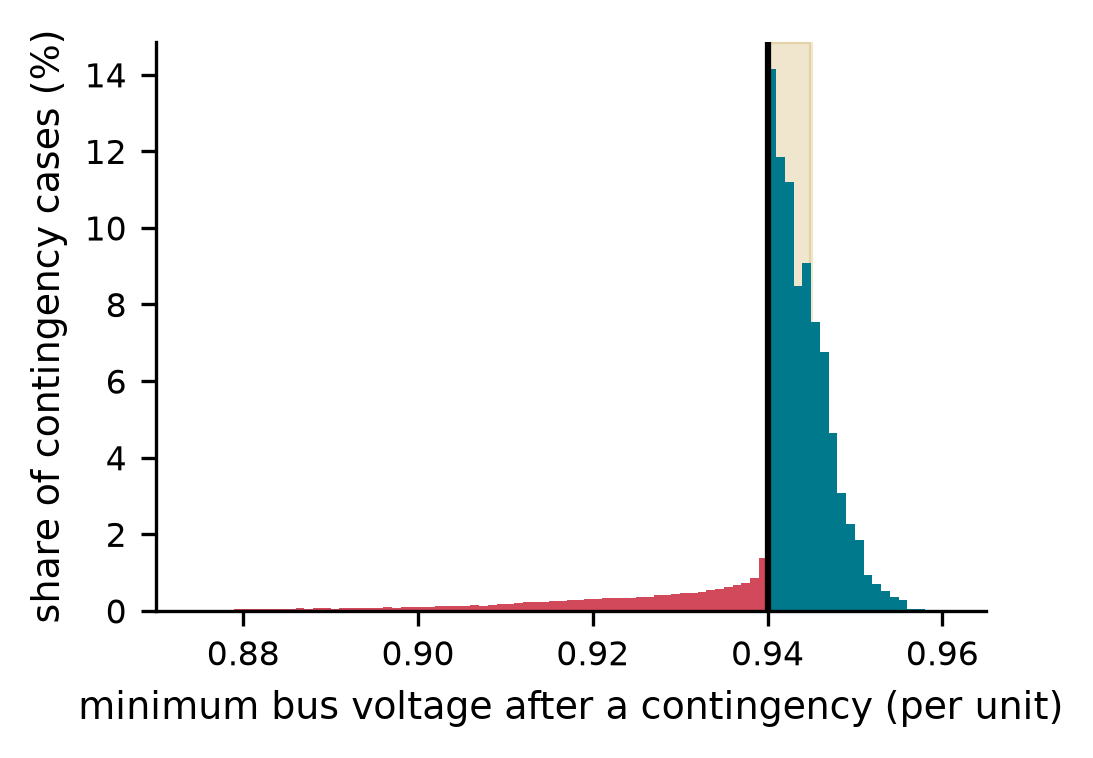
\includegraphics[width=0.5\textwidth]{data/sts_n13_fig4_boundary.png}
\caption{Minimum bus voltage after a contingency across 278,945 converged N-1 cases; anything left of the limit line is a violation. The shaded strip from [0.94, 0.945) contains 54.75\% of all cases, and the tallest 0.001 pu bin within it contains only 14.15\%. The x-axis is truncated at 0.87 pu, where 0.42\% of cases fall below it.}


\vspace*{1ex}
{\scriptsize Graph created by Rajan Saha using Matplotlib 3.11.1, 2026}
\label{fig:boundary}
\end{figure}


A case is escalated when the prediction lies within one band width above the 0.94 pu limit, since the band straddles the threshold. The gradient-boosted model's held-out band is only 0.0051 pu wide, but so much of the distribution sits just above 0.94 that this narrow window still escalates 54.25\% of all contingencies. As the band becomes larger, escalation moves closer to every case predicted at or above the limit, which for a perfect model is 83.74\% of all cases (or the saturation point).

To test if the generator setpoint values were the main reason the boundary mass was so high, I moved the lowest allowed generator setpoint and checked if the boundary mass near 0.94 changed as I had predicted in advance. My original predictions in Section~\ref{subsec:prereg} were chosen from knowing that a setpoint floor below the 0.94 limit is expected to have little to no effect on the boundary mass at 0.94, and floor above the limit pushes generator setpoints higher, so there should be fewer post-outage minimum voltages within [0.94, 0.945). After testing, 58.07\% of cases were within [0.94, 0.945) at 0.93, 56.86\% at 0.94, 32.95\% at 0.95, and 19.91\% at 0.96. All four of these were from the original data, and the 58.07\% (predicted range 50--62) and 19.91\% (predicted range 8--30) figures both fall into my predicted ranges. I then checked the new data to see if the result was similar, and it was, as at 0.93 there were 56.32\% of cases within 5 points of the 54.75\% figure from 0.94, and at 0.96 18.97\% was more than 5 points below the 33.36\% figure from 0.95, and both of these values passed the test, as shown in Table~\ref{tab:floor}. In addition, all three builds from the 0.95 setpoint averaged 32.29$\pm$0.77\%.

% ---------------------------------------------------------------------
% TABLE V (tab:floor) -- original build: data/sts_n11_dose_response.json
% (stored labels, on which the pre-registered verdict was decided);
% rebuilt: data/sts_n13_floor.json -> per_floor[];
% 0.95 replication average: data/sts_n13_floorrep.json -> across.
% ---------------------------------------------------------------------
\begin{table}[htbp]
\centering
\caption{Boundary mass (share of converged N-1 rows in [0.94, 0.945)) on case118 at four generator setpoint floors. Predictions for 0.93 and 0.96 were set in advance and tested on the original build, using labels stored before the switch-back fix; the rebuilt column re-applies the same pass/fail rules as a replication. $^{\ddagger}$One of three 0.95 rebuilt builds, which average 32.29$\pm$0.77\%. The gate results use the 0.94 build.}
\label{tab:floor}
\small
\setlength{\tabcolsep}{4pt}
\begin{tabular}{ccccc}
\toprule
Setpoint floor (pu) & Predicted (\%) & Original build (\%) & Rebuilt (\%) & Violation rate, rebuilt (\%) \\
\midrule
0.93 & 55 (50--62) & 58.07 & 56.32 & 16.35 \\
0.94 & --          & 56.86 & 54.75 & 16.26 \\
0.95 & --          & 32.95 & 33.36$^{\ddagger}$ & 14.81 \\
0.96 & 20 (8--30)  & 19.91 & 18.97 & 13.59 \\
\bottomrule
\end{tabular}

\vspace*{1ex}
{\scriptsize Table created by Rajan Saha using Python and \LaTeX, 2026}
\end{table}



\subsection{Coverage under N-2 outages}

I also tested whether the band that was calibrated on N-1 outages would still maintain its promise on N-2 contingencies. At the 0.90 target, the empirical coverage dropped from 0.9050 (N-1) to 0.8394 (N-2). Since my passing threshold, set from the pre-set formula, was 0.8861, the band, therefore, does not maintain its promise. In addition, the original build also failed, as it resulted in an empirical coverage of 0.8346 when the passing threshold was 0.8819. The missed rate for N-2 contingencies is 4.60$\pm$0.80\%, with no split being at or under 1\%, as shown in Table~\ref{tab:n2}. At the held-out point, the target coverage was 0.970, with the measured coverage of 0.9352 on N-2 compared to 0.9696 on N-1, and the missed rate was 1.40\%, with 3 of 5 splits having a sub-1\% missed rate.

% ---------------------------------------------------------------------
% TABLE VI (tab:n2) -- data/sts_n13_n2.json -> summary[family=histgb];
% threshold from data/sts_n13_verdicts.json -> COVERAGE_HOLDS_N2.
% ---------------------------------------------------------------------
\begin{table}[htbp]
\centering
\caption{histgb gate calibrated on N-1 data and tested on N-2 outages (50 random branch pairs per base case, no recalibration) on case118. Means $\pm$ standard deviation over five splits. The pass threshold from the pre-set formula at the 0.90 target was 0.8861.}
\label{tab:n2}
\small
\setlength{\tabcolsep}{5pt}
\begin{tabular}{lcccc}
\toprule
Target & N-1 coverage & N-2 coverage & N-2 missed (\%) & Splits $\le$1\% missed \\
\midrule
0.90     & 0.9050$\pm$0.0139 & 0.8394$\pm$0.0126 & 4.60$\pm$0.80 & 0/5 \\
held-out & 0.9696$\pm$0.0144 & 0.9352$\pm$0.0208 & 1.40$\pm$1.04 & 3/5 \\
\bottomrule
\end{tabular}

\vspace*{1ex}
{\scriptsize Table created by Rajan Saha using Python and \LaTeX, 2026}
\end{table}

% =====================================================================
\section{Discussion and limitations}
\label{sec:discussion}

Calibrated uncertainty, as well as making the decision of either outsourcing the problem or not to a more complex model \cite{desalvo2015} and providing the model with multiple choices \cite{angelopoulos2024,cortes2016,chow1970,elyaniv2010}, are existing methods. In this study, two things differ from that literature. First, I fall back to an exact solver instead of a more complex model, so the escalated case can be resolved, and second, I also explain why the speedup is capped, which is because most of the data is very close to the limit.

My approach differs from Manoharan's audited population control \cite{manoharan2026}, which is itself a form of distribution-free risk control \cite{bates2021}. That method uses a bound for the proportion of skipped cases that are unsafe, while the gate uses a margin of error that is subtracted from each prediction. This establishes the lower bound, since in split conformal prediction the claim of promise is accurate on average across several cases. If one demands perfect correctness per each case of cases with a distribution-free conditional coverage, then the resulting prediction intervals become infinitely wide, to the point where it becomes useless \cite{barber2021}.

The key findings obtained during the experiments relate to a network with a realistic topology and synthetic loads and generation. This escalation floor is set by how the distribution of the data occurs in relation to the 0.94 pu limit. For instance, in a regeneration of the IEEE 30-bus network that is thermally feasible in the base case, 7.10\% of contingencies fall just above the 0.94 pu limit, while another 15.38\% fall below it. For case118, 54.75\% fall just above the limit, and 16.26\% fall below it, which helps explain case30 having a 4.75 times speedup B while case118 only having 1.44. The original 30-bus system is thermally unrealistic, since it has 111.83\% line loading in its base case. 

After refitting the saved models to measure how deep the misses were, the results reproduced the original numbers exactly. This analysis was not pre-registered, and I did it after viewing the results. The gate typically misclassifies an unsafe case as safe when the true voltage is right under 0.94 pu. On case118, the median miss was 0.00183 pu below 0.94, with 77.1\% of misses being within 0.005 pu of the limit, with case30 and case24 showing a similar pattern. The worst miss from case118 was 0.0528 pu below the 0.94 limit. On the 3 networks (case118, case24, case30), when the worst split occurred, the inner tuning split chose the lowest target and made the band width small compared to the other splits.

In the sampled population, 28.73\% of bases (80{,}130 rows total) already have one generator out of service before the branch outage. Moreover, mathematical proof is not capable of guaranteeing the safety of N-2 outages where two branches fail together because the use of conformal prediction assumes that the data is exchangeable with the calibration set \cite{vovk2005}. Weighted conformal prediction relaxes exchangeability in an instance where there is a shift in the covariate distribution and the likelihood ratio between the two distributions is either known or can be estimated \cite{tibshirani2019}. However, this ratio only exists when the shifted distribution is absolutely continuous relative to the calibration distribution, which is not the case for N-2 outages. Also, I only checked if the final voltage was too low, not for thermal overheating, over-voltage, or whether or not the grid crashed in the first place, which is called dynamic stability. Lastly, all of the testing data were obtained by making slight modifications to the same pre-contingency grid setup. Therefore, there is some uncertainty as to how often the models should be recalibrated due to changes in the seasons and changes in demand. This study covered 4 grids, used synthetic grid load data, never checked the buses that were cut off from the slack bus, used six post hoc decisions, and only tested the solver speed on one computer. In addition, 43,283 of the 278,945 converged case118 rows have a true minimum voltage within $10^{-3}$ pu of the 0.94 limit (the safe/violation label is only as accurate as the switch-back loop's $10^{-3}$ pu tolerance).

This paper only reports some of the pre-registered experiments in full, and the remaining verdicts include SAFER-IL (missing at most 1\% of violations on Illinois in at least 4 of 5 splits; failed), SAFER (missing at most 1\% of violations in at least 4 of 5 splits on the 0.95-floor data; failed), FASTER (having a higher speedup B on 0.95 than 0.94 and catching more violations than the fixed list at the same solve budget by more than the larger standard deviation — the speedup B part passed while the catch-rate part tied, so this experiment failed), SHIFT-ADVANTAGE (beating the fixed list when trained on 0.94-floor data and tested on 0.95-floor data by more than the larger standard deviation; failed), MONDRIAN-BEATS-STATIC (a per-group conformal gate that was tested compared with static ranking — while it did tie on the original build, the gate won on the rebuilt version as the gap was more than the larger standard deviation), SAFETY-CHANGED (tests whether the missed rate changed between builds; it does not), and MISMATCH-DRIVES-DRIFT-GAP (tests if the incorrect input voltages in the original data result in the gate to miss more violations; it does not).


\subsection{Physics-feature ablation}\label{subsec:ablation}

I tested five different setups on the original labels with agg\_loading being left out of all the runs: baseline, +F1 (add pre-outage branch flows on the outaged element), +F1+F2 (add F1 and the full pre-outage loading vector), +F1+F3 (add F1 and the LODF rows), and +F1+F2+F3+F4 (add F1, F2, F3, and electrical distance F4). For each configuration, ridge and histogram-based gradient boosting both had hyperparameters re-searched and fixed. The best configurations (with hyperparameters re-searched) had a MAE of $0.00371 \pm 0.00010$ for ridge and $0.00153 \pm 0.00011$ for histgb. The additional features contribute no meaningful increase in performance compared to the basic ones, as the benefit from the addition of the features is less than the seed standard deviation.

The one negative outcome obtained here is that including F2 (the entire vector of pre-outage loadings) worsens ridge's results, as MAE increases by +10.82\% (baseline $0.003754 \pm 0.000133$ to +F1+F2 $0.004161 \pm 0.000247$ in the re-searched runs), which is bigger than the seed variation. 

To investigate further, I compared the basic model, the model with real F1 data, and a model with shuffled F1 data. The shuffled data had a higher error rate (worse) than the real F1 for histgb across 4 of 5 seeds, with the average difference across all 5 being $(1.83\pm2.51)\times 10^{-5}$, but this difference is small enough that it falls within normal seed variation, as the mean (1.83) is smaller than its spread (2.51).



% =====================================================================
\section{Conclusion and future work}
\label{sec:conclusion}

On case118, the gate misses 1.14\% of violations, has a 1.44 times speedup B, and solved 70.9\% of the cases. On case118 and Illinois-200, the gate ties the history baseline's performance and beats it on case30 and case24. The pre-registered primary test on Illinois-200 became a tie after the post hoc exclusion of trafo 63, and case24's results come from a post hoc tolerance rule. The gate is unable to maintain its coverage promise on N-2 under-voltage contingencies, as the coverage dropped to 0.8394, which is well under the passing threshold of 0.8861. The floor experiment on the original data supported my predictions, and it was replicated on the fixed data. In conclusion, speedup is limited by the near-limit mass on case118 and from the violation rate on case24. Histgb ranking only beats fixed static ranking at small solve budgets on case118 (Table~\ref{tab:budget}). On case30 COND-HIST only caught 89.81\% (Table~\ref{tab:networks}), and the reasoning behind this weaker performance is an open question. Future work includes testing more grids, using real load data, calibrating the gate on N-2 data, and providing per-group guarantees rather than just on average guarantees.


\section*{Acknowledgments}

This paper has been written as part of the Boston University RISE data science practicum. I would like to thank the program and the teaching fellows and staff, including Dr. Eugene Pinsky, Dr. Indrajit Kalita, and teaching fellows Tharunya Katikireddy, Yaswanth Anumolu, Victor Wang and Adrish Dey.
% =====================================================================
% References. arXiv entries verified in notes/prior-art.md; the classic and
% software entries were fetch-verified on 2026-07-21 (dblp, IEEE Xplore,
% Oxford Academic, NeurIPS proceedings, JMLR, UW test-case archive); the two
% ALT conference entries (cortes2016, desalvo2015) on 2026-07-23 (Crossref + dblp;
% Springer chapter pages behind an auth wall); bates2021 from the publisher
% PDF; tibshirani2019 on 2026-07-26 (NeurIPS proceedings page + ACM DL);
% angelopoulos2024, christianson2025 and ansi2020 on 2026-07-29 (medRxiv full
% text, proceedings.mlr.press/v283/christianson25a.html, and the NEMA official
% excerpt respectively). No field is filled from memory.
% NERC (nerc) confirmed against nerc.com as TPL-001-5.1, effective
% 2023-07-01; verified 2026-09-15 (nerc.com PDF and standard page, notes/prior-art.md section 9.10).
% =====================================================================
\newpage
\thispagestyle{empty}
\singlespacing
\begin{thebibliography}{26}

\bibitem{nerc} \textit{Transmission System Planning Performance Requirements}, NERC Reliability Standard TPL-001-5.1, North American Electric Reliability Corporation, Atlanta, GA, USA, eff. Jul. 1, 2023.

\bibitem{bates2021} S. Bates, A. Angelopoulos, L. Lei, J. Malik, and M. I. Jordan, ``Distribution-free, risk-controlling prediction sets,'' \textit{J. ACM}, vol. 68, no. 6, pp. 1--34, Dec. 2021, doi: 10.1145/3478535.

\bibitem{manoharan2026} J. Manoharan, ``Audited selective verification for risk-controlled N-1 thermal contingency screening under deployment shift,'' arXiv:2607.13221, Jul. 2026.

\bibitem{alcantara2026} A. Alc\'antara and S. Chatzivasileiadis, ``Trustworthiness layer for foundation models in power systems: Application to N-k contingency screening,'' arXiv:2602.07995v2, Apr. 2026.

\bibitem{christianson2025} N. Christianson, W. Cui, S. Low, W. Yang, and B. Zhang, ``Fast and reliable N-k contingency screening with input-convex neural networks,'' in \textit{Proc. 7th Annu. Learn. Dynamics Control Conf. (L4DC)}, ser. PMLR, vol. 283, 2025, pp. 527--539.

\bibitem{pypower} R. Lincoln, ``PYPOWER,'' (a port of MATPOWER to the Python programming language). [Online]. Available: \url{https://github.com/rwl/PYPOWER} (accessed October 16, 2026).

\bibitem{ejebe1979} G. C. Ejebe and B. F. Wollenberg, ``Automatic contingency selection,'' \textit{IEEE Trans. Power App. Syst.}, vol. PAS-98, no. 1, pp. 97--109, Jan. 1979, doi: 10.1109/TPAS.1979.319518.

\bibitem{case118} R. Christie, ``118 bus power flow test case,'' Power Systems Test Case Archive, Univ. of Washington, Seattle, WA, USA, 1993. [Online]. Available: \url{https://labs.ece.uw.edu/pstca/pf118/pg_tca118bus.htm}

\bibitem{illinois200} A. B. Birchfield, T. Xu, K. M. Gegner, K. S. Shetye, and T. J. Overbye, ``Grid Structural Characteristics as Validation Criteria for Synthetic Networks,'' \textit{IEEE Transactions on Power Systems}, vol. 32, no. 4, pp. 3258--3265, July 2017, doi: 10.1109/TPWRS.2016.2616385.

\bibitem{case30} O. Alsac and B. Stott, ``Optimal Load Flow with Steady-State Security,'' \textit{IEEE Transactions on Power Apparatus and Systems}, vol. PAS-93, no. 3, pp. 745--751, May/June 1974, doi: 10.1109/TPAS.1974.293972.

\bibitem{case24} IEEE Reliability Test System Task Force of the Applications of Probability Methods Subcommittee, ``IEEE Reliability Test System,'' \textit{IEEE Transactions on Power Apparatus and Systems}, vol. PAS-98, no. 6, pp. 2047--2054, Nov./Dec. 1979, doi: 10.1109/TPAS.1979.319398.

\bibitem{pandapower} L. Thurner, A. Scheidler, F. Sch\"afer, \textit{et al.}, ``pandapower---an open-source Python tool for convenient modeling, analysis, and optimization of electric power systems,'' \textit{IEEE Trans. Power Syst.}, vol. 33, no. 6, pp. 6510--6521, Nov. 2018, doi: 10.1109/TPWRS.2018.2829021.

\bibitem{matpower} R.~D. Zimmerman, C.~E. Murillo-S{\'a}nchez, and R.~J. Thomas, ``MATPOWER: Steady-State Operations, Planning, and Analysis Tools for Power Systems Research and Education,'' {\em IEEE Transactions on Power Systems}, vol.~26, no.~1, pp.~12--19, Feb. 2011, doi:~10.1109/TPWRS.2010.2051168.



\bibitem{sklearn} F. Pedregosa \textit{et al.}, ``Scikit-learn: Machine learning in Python,'' \textit{J. Mach. Learn. Res.}, vol. 12, pp. 2825--2830, 2011.

\bibitem{lei2018} J. Lei, M. G'Sell, A. Rinaldo, R. J. Tibshirani, and L. Wasserman, ``Distribution-free predictive inference for regression,'' \textit{J. Amer. Statist. Assoc.}, vol. 113, no. 523, pp. 1094--1111, 2018, doi: 10.1080/01621459.2017.1307116.

\bibitem{vovk2005} V. Vovk, A. Gammerman, and G. Shafer, \textit{Algorithmic Learning in a Random World}. New York, NY, USA: Springer, 2005, doi: 10.1007/b106715.
  
\bibitem{angelopoulos2023} A. N. Angelopoulos and S. Bates, ``Conformal prediction: A gentle introduction,'' \textit{Found. Trends Mach. Learn.}, vol. 16, no. 4, pp. 494--591, 2023, doi: 10.1561/2200000101.

\bibitem{romano2019} Y. Romano, E. Patterson, and E. J. Cand\`es, ``Conformalized quantile regression,'' in \textit{Adv. Neural Inf. Process. Syst. (NeurIPS)}, vol. 32, 2019.

\bibitem{geifman2017} Y. Geifman and R. El-Yaniv, ``Selective classification for deep neural networks,'' in \textit{Adv. Neural Inf. Process. Syst. (NeurIPS)}, vol. 30, 2017.

\bibitem{chow1970} C. Chow, ``On optimum recognition error and reject tradeoff,'' \textit{IEEE Trans. Inf. Theory}, vol. 16, no. 1, pp. 41--46, Jan. 1970, doi: 10.1109/TIT.1970.1054406.

\bibitem{barber2021} R. F. Barber, E. J. Cand\`es, A. Ramdas, and R. J. Tibshirani, ``The limits of distribution-free conditional predictive inference,'' \textit{Inf. Inference: J. IMA}, vol. 10, no. 2, pp. 455--482, 2021.

\bibitem{tibshirani2019} R. J. Tibshirani, R. Foygel Barber, E. J. Cand\`es, and A. Ramdas, ``Conformal prediction under covariate shift,'' in \textit{Adv. Neural Inf. Process. Syst. (NeurIPS)}, vol. 32, 2019.

\bibitem{desalvo2015} G. DeSalvo, M. Mohri, and U. Syed, ``Learning with deep cascades,'' in \textit{Algorithmic Learning Theory (ALT)}, ser. Lecture Notes in Comput. Sci., vol. 9355. Cham, Switzerland: Springer, 2015, pp. 254--269, doi: 10.1007/978-3-319-24486-0\_17.

\bibitem{angelopoulos2024} A. N. Angelopoulos \textit{et al.}, ``Conformal triage for medical imaging AI deployment,'' medRxiv preprint, 2024, doi: 10.1101/2024.02.09.24302543.

\bibitem{cortes2016} C. Cortes, G. DeSalvo, and M. Mohri, ``Learning with rejection,'' in \textit{Algorithmic Learning Theory (ALT)}, ser. Lecture Notes in Artif. Intell., vol. 9925. Cham, Switzerland: Springer, 2016, pp. 67--82, doi: 10.1007/978-3-319-46379-7\_5.

\bibitem{elyaniv2010} R. El-Yaniv and Y. Wiener, ``On the foundations of noise-free selective classification,'' \textit{J. Mach. Learn. Res.}, vol. 11, pp. 1605--1641, 2010.

\end{thebibliography}
\thispagestyle{empty}

\end{document}